%%%%%%%%%%%%%%%%%%%%%%%%%%%%%%%%%%%%%%%%%
% Simple Sectioned Essay Template
% LaTeX Template
%
% This template has been downloaded from:
% http://www.latextemplates.com
%
% Note:
% The \lipsum[#] commands throughout this template generate dummy text
% to fill the template out. These commands should all be removed when 
% writing essay content.
%
%%%%%%%%%%%%%%%%%%%%%%%%%%%%%%%%%%%%%%%%%

%----------------------------------------------------------------------------------------
%	PACKAGES AND OTHER DOCUMENT CONFIGURATIONS
%----------------------------------------------------------------------------------------

\documentclass[12pt]{article} % Default font size is 12pt, it can be changed here

\usepackage{geometry} % Required to change the page size to A4
\geometry{a4paper} % Set the page size to be A4 as opposed to the default US Letter

\usepackage{graphicx} % Required for including pictures

\usepackage{float} % Allows putting an [H] in \begin{figure} to specify the exact location of the figure
\usepackage{wrapfig} % Allows in-line images such as the example fish picture

\usepackage{lipsum} % Used for inserting dummy 'Lorem ipsum' text into the template
\usepackage{subfigure}

\usepackage{url}

\linespread{1.2} % Line spacing

%\setlength\parindent{0pt} % Uncomment to remove all indentation from paragraphs

\graphicspath{{Pictures/}} % Specifies the directory where pictures are stored

\begin{document}

%----------------------------------------------------------------------------------------
%	TITLE PAGE
%----------------------------------------------------------------------------------------

\begin{titlepage}

\newcommand{\HRule}{\rule{\linewidth}{0.5mm}} % Defines a new command for the horizontal lines, change thickness here

\center % Center everything on the page

\textsc{\LARGE Universit\'a Tor Vergata}\\[1.5cm] % Name of your university/college
\textsc{\Large Corso di Laurea di Ingegneria Informatica}\\[0.5cm] % Major heading such as course name
\textsc{\large A.A. 2015-2016}\\[0.5cm] % Minor heading such as course title

\HRule \\[0.4cm]
{ \huge \bfseries Mobile Sniffing Tool}\\[0.4cm] % Title of your document
{ \bfseries Progetto di Sicurezza Informatica e Internet}\\[0,4cm]
\HRule \\[1.5cm]

\begin{minipage}{0.4\textwidth}
\begin{flushleft} \large
\emph{Autori:}\\
Paolo \textsc{Salom\'e}\\
Stefano \textsc{Agostini} % Your name
\end{flushleft}
\end{minipage}
~
\begin{minipage}{0.4\textwidth}
\begin{flushright} \large
\emph{Supervisori:}\\
Prof. Giuseppe \textsc{Italiano}\\ 
Dr. Marco \textsc{Querini}  % Supervisor's Name
\end{flushright}
\end{minipage}\\[8,5cm]

{\large \today}\\[3cm] % Date, change the \today to a set date if you want to be precise

%\includegraphics{Logo}\\[1cm] % Include a department/university logo - this will require the graphicx package

\vfill % Fill the rest of the page with whitespace

\end{titlepage}

%----------------------------------------------------------------------------------------
%	TABLE OF CONTENTS
%----------------------------------------------------------------------------------------

\tableofcontents % Include a table of contents

\newpage % Begins the essay on a new page instead of on the same page as the table of contents 

%----------------------------------------------------------------------------------------
%	INTRODUCTION
%----------------------------------------------------------------------------------------

\section{Introduzione} % Major section

Nella societ\'a odierna vi \'e un larga diffusione di applicazioni mobile di messagistica che espongono implicitamente gli utenti a problematiche riguardanti la privacy. Infatti fino a qualche mese fa i dati in transito di Whatsapp (e.g.) erano in chiaro e quindi accedibili facilmente da chiunque utilizzasse una qualsiasi applicazione per lo sniffing (e.g. Whireshark). Tuttavia attualmente molte delle applicazioni di messaggistica hanno rimediato interamente o parzialmente utilizzando tecniche di crittografia end-to-end. 
L'obiettivo del nostro progetto \'e la realizzazione di una applicazione per sistemi mobile Android che all'interno di una certa rete wifi catturi i dati in transito e li filtri in base ad un flag. In tal modo ci preponiamo l'obiettivo di isolare i pacchetti dati per ogni applicazione di messaggistica presa in considerazione e analizzarli.
 
%------------------------------------------------

%\subsection{Subsection 1} % Sub-section

%\lipsum[1] % Dummy text

%------------------------------------------------

%\subsection{Subsection 2} % Sub-section

%\lipsum[2] % Dummy text

%------------------------------------------------

%\subsubsection{Subsubsection 1} % Sub-sub-section

%\lipsum[3] % Dummy text

%\begin{figure}[H] % Example image
%\center{
\includegraphics[width=0.5\linewidth]{placeholder}}
%\caption{Example image.}
%\label{fig:speciation}
%\end{figure}

%------------------------------------------------

%\subsubsection{Subsubsection 2} % Sub-sub-section

%\lipsum[4] % Dummy text

%----------------------------------------------------------------------------------------
%	MAJOR SECTION 1
%----------------------------------------------------------------------------------------

\section{Descrizione dell'Applicazione} % Major section

Per realizzare uno \textit{sniffer Android} c'erano due strade alternative da poter seguire: sfruttare le \textit{Android VPN} oppure utilizzare l'eseguibile \textit{C tcpdump}. L'approccio \textit{Android VPN} consiste nella creazione di un'interfaccia \textit{VPNService}, gestita da una applicazione in \textit{userspace}, che una volta attivata forza tutto il traffico del \textit{device} ad attraversarla. Tuttavia questo approccio non permette la cattura di pacchetti appartenenti a dispositivi diversi da quello ospitante l'applicazione. Per utilizzare il secondo approccio \'e necessario che il dispositivo abbia i permessi di \textit{root} in quanto verr\'a eseguito uno \textit{script bash tcpdump}, il quale si occuper\'a di catturare i pacchetti. Inoltre questa libreria permette di sfruttare la scheda di rete in uso in varie modalit\'a (e.g. \textit{promiscous mode, monitor mode}) qualora il dispositivo lo consenta. La possibilit\'a di sfruttare a pieno le potenzialit\'a della scheda di rete ci ha indotto a scegliere \textit{tcpdump}.     

%------------------------------------------------

\subsection{Tcpdump} % Sub-section

\textit{Tcpdump} \'e un eseguibile \textit{command-line} basato su \textit{libpcap}, una libreria \textit{C} portabile che offre \textit{API} utili per la cattura del traffico di rete. Abbiamo deciso di utilizzare \textit{tcpdump} anzich\'e direttamente le \textit{API} di \textit{libpcap} poich\'e esso si presta maggiormente all'esecuzione su piattaforma \textit{Android} (si esegue direttamente su \textit{bash}).

Il comando \textit{bash} dell'eseguibile \textit{tcpdump} permette l'inserimento di alcuni parametri che consentono la visualizzazione dei pacchetti in vari formati. Nel caso della nostra applicazione utilizziamo i seguenti parametri:

\begin{itemize}
\item \textbf{-i} : seguito dal nome dell'interfaccia, per specificare dove porsi in ascolto (e.g. wlan0)
\item \textbf{-XX} in alternativa a \textbf{-A}: il primo stampa l'header di ogni pacchetto e i dati in esadecimale e \textit{ASCII} mentre il secondo non stampa l'esadecimale
\item \textbf{-tttt}: stampa la data corrente davanti l'header di ogni pacchetto in formato \textit{YYYY-MM-DD hh:mm:ss:dddddd}
\end{itemize}

Di seguito inseriamo un pacchetto di esempio stampato da bash come risultato del comando \textit{sudo tcpdump -i wlan0 -XX -tttt} (figure \ref{fig:XX}) e del comando \textit{sudo tcpdump -i wlan0 -A -tttt} (figure \ref{fig:A}).

\begin{figure}[H] % Example image
\center{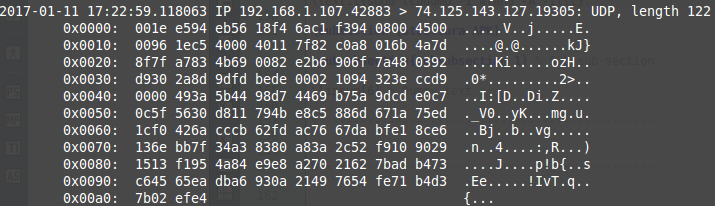
\includegraphics[scale=0.6]{tcpdump_XX.png}}
\caption{Con opzione -XX}\label{fig:XX}
\end{figure}

\begin{figure}[H] % Example image
\center{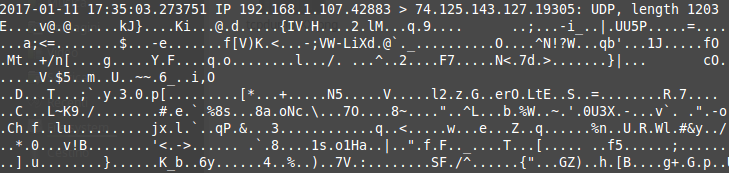
\includegraphics[scale=0.6]{tcpdump_A.png}}
\caption{Con opzione -A}\label{fig:A}
\end{figure}

\newpage
\subsection{Struttura APK}
La nostra \textit{APK} si compone di due \textit{Activity} e due \textit{Service}:

\begin{itemize}
\item L'\textit{Activity} di cattura espone un'interfaccia semplice per impostare la modalit\'a di cattura (specificare il \textit{flag} \textit{hex mode}). Successivamente l'utente pu\'o specificare il nome del file sul quale vuole che vengano salvati i pacchetti. Infine \'e possibile attivare il servizio di cattura.
\item L'\textit{Activity} di filtraggio si occupa di fornire all'utente un elenco dei file contenenti i pacchetti, salvati dall'applicazione stessa nelle precedenti catture. Selezionato il file da elenco \'e possibile inserire la parola chiave di ricerca. Mediante il servizio di filtraggio \'e vengono scanditi i pacchetti e visualizzati in una lista soltanto quelli contenenti la parola desiderata.
\item Il \textit{Service} di cattura si occupa dell'invocazione del comando \textit{tcpdump} con le opzioni e il nome del file passati dall'\textit{Activity} di cattura, redirezionando l'output su quest'ultimo. Quando questo servizio viene interrotto si esegue il comando bash \textit{pkill tcpdump} per terminare il comando dello \textit{sniffer}. 
\item Il \textit{Service} di filtraggio agisce sul file selezionato esaminando ogni pacchetto e inserendolo in una lista visualizzata a schermo solo se contiene la \textit{keyword} fornita, all'interno dell'\textit{header} o del \textit{body}.
\end{itemize}
 
Di seguito inseriamo degli \textit{screen} dell'applicazione appena descritta (figure \ref{fig:apk}).
 
 
\begin{figure}[htbp]
\centering%
\subfigure[Activity di cattura\label{fig:apk1}]%
{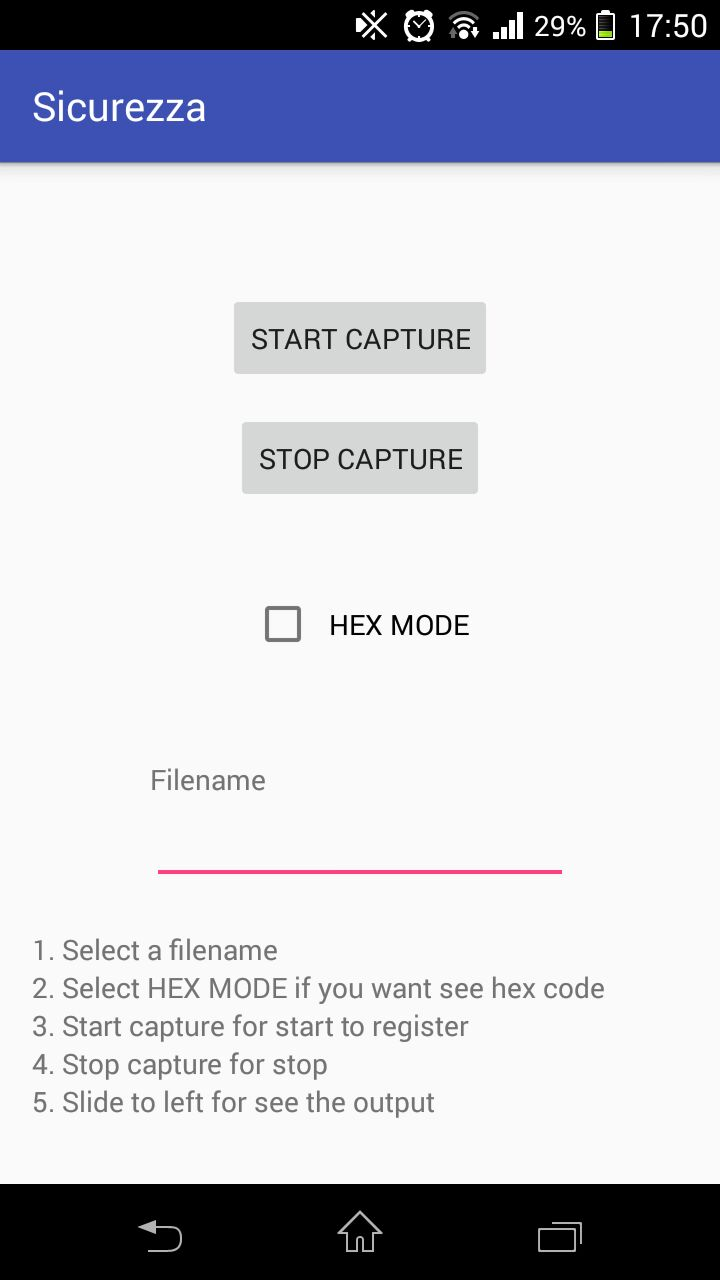
\includegraphics[scale=0.2]{./activity1.jpeg}}\qquad\qquad
\subfigure[Activity di filtraggio\label{fig:apk2}]%
{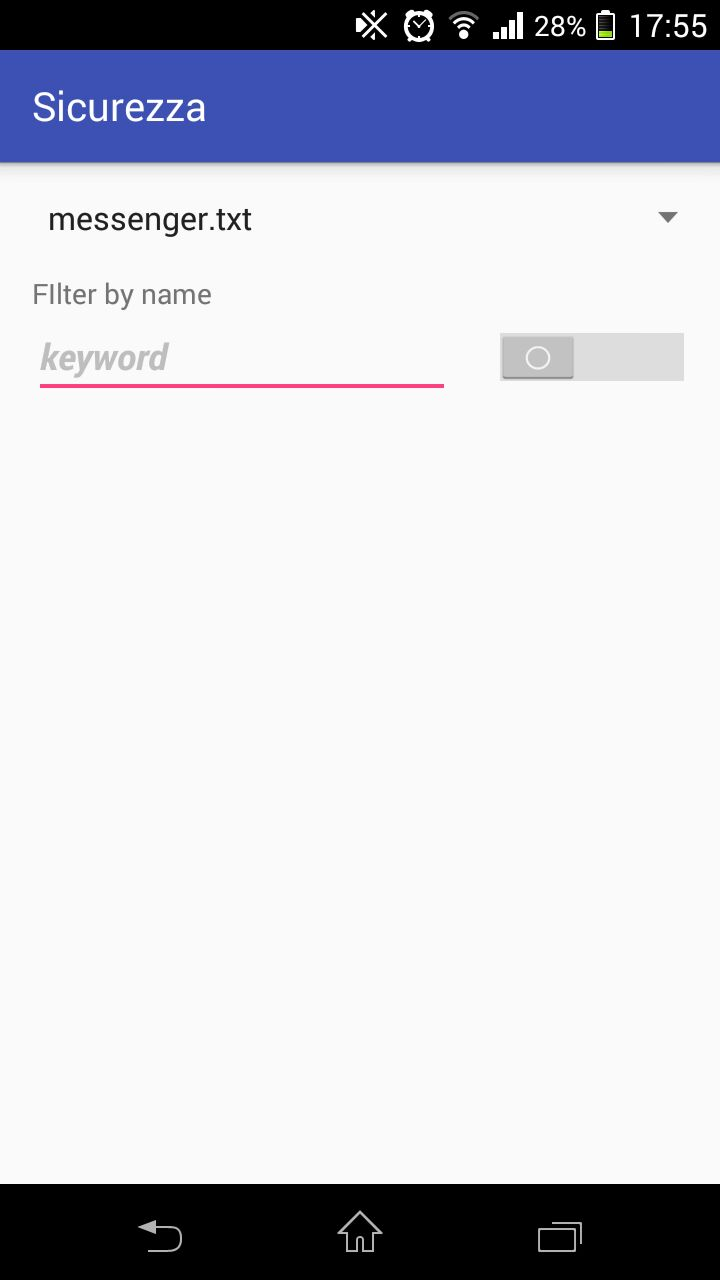
\includegraphics[scale=0.2]{./activity2.jpeg}}\qquad\qquad
\\
\subfigure[Lista di file\label{fig:filelist}]%
{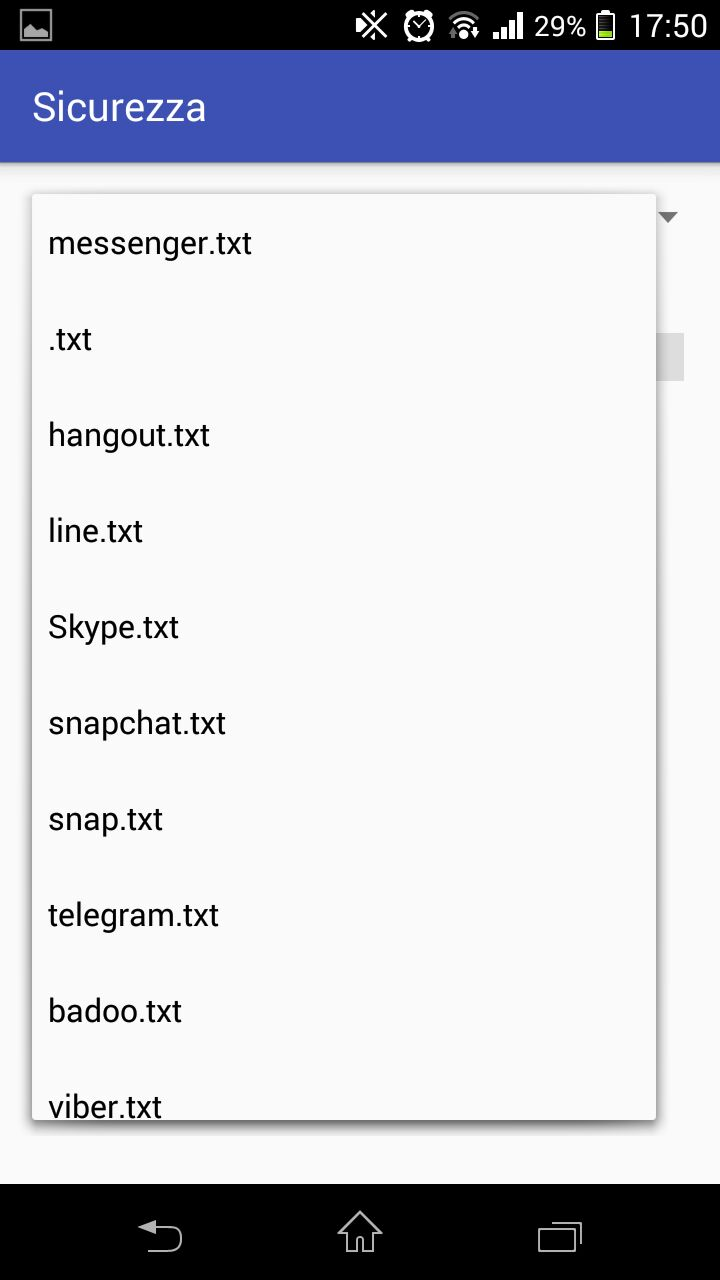
\includegraphics[scale=0.2]{./filelist.jpeg}}\qquad\qquad
\subfigure[Pacchetti filtrati\label{fig:apk2active}]%
{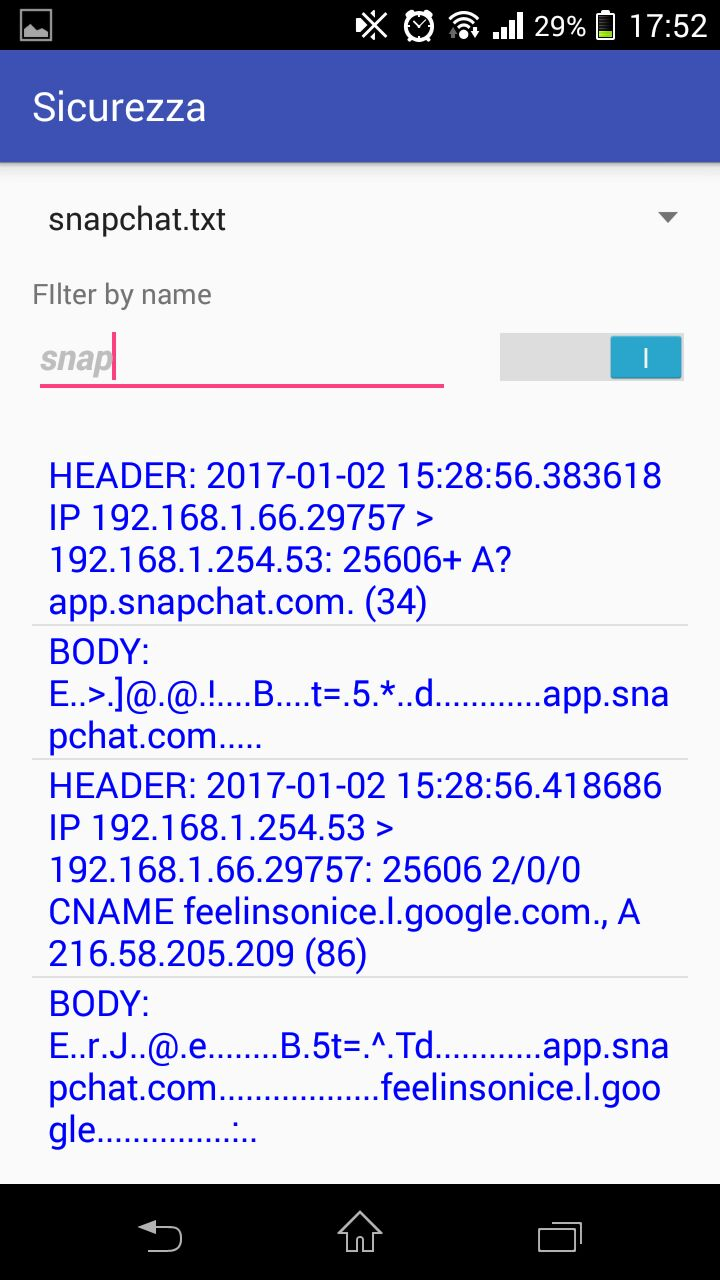
\includegraphics[scale=0.2]{./activity2active.jpeg}}
\caption{Pagine dell'applicazione\label{fig:apk}}
\end{figure} 
 
\subsubsection{Activity di cattura} % Sub-sub-section
L'\textit{Activity} di cattura \'e implementata dalla classe \textit{MainActivity} e realizza la schermata iniziale per l'utente. Essa estende la classe \textit{AppCompatActivity} ed effettua l'\textit{override} dei metodi \textit{onCreate} e \textit{onTouchEvent}. Quest'ultimo implementa un \textit{listener} che, a seguito del primo tocco dell'utente, esegue le seguenti operazioni:

\begin{itemize}
\item Salva la posizione iniziale al tocco.
\item Al rilascio calcola il \textit{delta} rispetto alla posizione iniziale.
\item Se il \textit{delta} \'e maggiore di 400 \textit{pixel} verso sinistra invoca l'\textit{Activity} di filtraggio.  
\end{itemize}

Infine ci sono i due metodi legati ai bottoni di \textit{start} e \textit{stop} del servizio di cattura. Il metodo \textit{startclick} esegue i seguenti passi all'invocazione:

\begin{itemize}
\item Cerca il riferimento all'\textit{editText} contenente il nome del file in cui salvare i pacchetti catturati.
\item Verifica lo stato della \textit{checkbox} relativa alla modalit\'a \textit{hex mode}.
\item Crea l'\textit{Intent} da passare al servizio di cattura.
\item Utilizza il metodo \textit{putExtra} dell'\textit{Intent} per passare i parametri di cattura al servizio (\textit{path} del file e eventualmente il \textit{flag hex}).
\end{itemize}

Il metodo \textit{stopclick} crea un nuovo \textit{Intent} per il servizio di cattura avviato precedentemente e invoca il metodo \textit{stopService} per forzarne l'interruzione.

\subsubsection{Activity di filtraggio}
Questa \textit{Activity} \'e implementata dalla classe \textit{SecondActivity} la quale estende la classe \textit{AppCompatActivity}. Il metodo \textit{OnCreate} effettua le seguenti operazioni:

\begin{itemize}
\item Recupera lo \textit{switch} relativo all'attivazione del servizio di filtraggio.
\item Inizializza lo stato dello \textit{switch} a \textit{false}.
\item Fa l'\textit{override} del metodo \textit{OnCheckedChanged}, il quale rappresenta il \textit{listener} dello \textit{switch}. Quest'ultimo:
\begin{itemize}
\item Se lo \textit{switch} \'e \textit{checked} inizializza la \textit{ListView} che apparir\'a a schermo e l'\textit{Adapter} ad essa associato. Successivamente invoca il metodo \textit{viewFile} di cui parleremo in seguito.
\item Se lo \textit{switch} \'e \textit{unchecked} invoca il metodo \textit{stopServ}.
\end{itemize}
\item Preleva tutti i file relativi alle precedenti registrazioni di pacchetti fatti dall'applicazione. I file sono raggruppati in una cartella sul dispositivo.
\item Prelevati i file questi vengono inseriti in una lista di stringhe. Quest'ultima verr\'a associata con un \textit{adapter} ad uno \textit{spinner} per consentire all'utente la selezione di un file.
\end{itemize}

Il metodo \textit{viewFile} effettua le seguenti operazioni:

\begin{itemize}
\item Preleva il nome del file dallo \textit{Spinner} ed il filtro.
\item Crea l'\textit{Intent} relativo al servizio di filtraggio ed aggiunge come parametri il \textit{filepath} ed il \textit{filter}.
\item Invoca il metodo \textit{startService} con parametro l'\textit{Intent} appena creato.
\end{itemize}

Il metodo \textit{stopServ} crea un nuovo \textit{Intent} per il servizio di filtraggio avviato precedentemente e invoca il metodo \textit{stopService} per forzarne l'interruzione.

Questa \textit{Activity} utilizza un \textit{BroadcastReceiver} per ricevere i dati elaborati dal servizio invocato. Di questo \textit{Receiver} viene fatto l'\textit{override} del metodo \textit{onReceive} il quale, in ricezione dei dati inviati dal servizio, aggiorna la \textit{ListView} presente nell'\textit{Activiy} stessa. Per utilizzare il \textit{BroadcastReceiver} col metodo \textit{onReceive} esso deve essere registrato mediante il metodo \textit{onResume}, il quale accetta un \textit{flag} per identificare gli \textit{Intent} da gestire (nel nostro sistema \textit{filterMessage}). D'altro canto il metodo \textit{onPause} serve a deregistrare il \textit{BroadcastReceiver} quando l'\textit{Activity} \'e in pausa.

Infine \'e implementato il metodo \textit{onTouchEvent} che si comporta esattamente come quello dell'\textit{Activity} precedentemente illustrata.

\subsubsection{Service di cattura}
Questo servizio \'e implementato dalla classe \textit{RegisterService}. Nel metodo \textit{onStartCommand} viene avviato lo \textit{sniffer} in seguito ai seguenti passi:

\begin{itemize}
\item Vengono estratti dall'\textit{Intent} passato dalla \textit{MainActivity} il \textit{path} del file ed eventualmente il \textit{flag} contenente l'\textit{hex mode}.
\item Vengono preparati i comandi da eseguire su \textit{bash} ovvero \textbf{su} per garantire i dovuti permessi di \textit{superuser} e il comando \textbf{tcpdump}.
\item Viene creato ed eseguito un processo \textit{bash}.
\item Viene effettuato un collegamento con l'\textit{OutputStream} del processo e vengono scritti i comandi da eseguire preparati in precedenza.
\item Al termine della scrittura viene opportunamente chiuso il collegamento con l'\textit{OutputStream} del processo.
\end{itemize}

Il metodo \textit{onDestroy} ha una struttura simile al metodo \textit{onStartCommand}, con la differenza nei comandi da eseguire su \textit{bash}. Esegue la terminazione dei processi precedentemente avviati tramite il comando \textbf{pkill tcpdump}. Infine termina il servizio tramite la chiamata al metodo \textit{this.stopSelf}. 

\subsubsection{Service di filtraggio}
La classe \textit{FilterService}, a differenza del \textit{Service} di cattura, \'e un \textit{IntentService}. Un \textit{Service} di questo tipo riesce ad eseguire richieste asincrone fornite dal \textit{Client} tramite un suo \textit{working thread}, diverso dal \textit{main thread} dell'applicazione. In tal modo si alleggerisce del lavoro il \textit{main thread} il quale pu\'o nel frattempo occuparsi di altro. Inoltre un \textit{IntentService} \'e in grado di eseguire pi\'u richieste, accodandole una dopo l'altra.

Abbiamo deciso di utilizzare questa soluzione poich\'e filtrare file di grandi dimensioni (come il caso di file contenenti pacchetti dati) avrebbe potuto causare attese molto lunghe e nei casi peggiori ledere la stabilit\'a dell'applicazione, causandone persino il \textit{chash}.

Il metodo \textit{onHandleIntent} si preoccupa di innescare il \textit{working thread} all'arrivo dell'\textit{Intent}, il quale esegue i seguenti passi:

\begin{itemize}
\item Recupera dall'\textit{Intent} inviato dall'\textit{Activity} di filtraggio il \textit{path} del file e il \textit{filter}.
\item Apre il file per collegarlo ad un oggetto \textit{BufferedReader}.
\item Vengono definite due stringhe utili ad identificare l'\textit{header} di ogni pacchetto: esse sono \textit{"IP" e "ARP"} poich\'e qualsiasi pacchetto nell'\textit{header} ha per identificativo anche il relativo protocollo di rete. Inoltre vengono inizializzate come stringhe vuote \textit{header e body} utili a contenere l'\textit{header} e il \textit{body} del pacchetto corrente.
\item Viene letto il file riga per riga ed ognuna di queste viene concatenata alla stringa \textit{header} se contiene \textit{"IP" o "ARP"} e nel caso contrario viene concatenata alla stringa \textit{body}.
\item Ogni volta che viene idenficato un nuovo \textit{header} vengono controllate le stringe \textit{header e body} relative al pacchetto precedente e, nel caso contengano la stringa \textit{filter}, allora verra invocata la \textit{sendBroadcast} con queste come parametri. Dopodich\'e viene azzerata la stringa \textit{body} e assegnato l'\textit{header} appena identificato alla stringa \textit{header}.
\item Al termine del file viene chiuso il \textit{BufferedReader}. 
\end{itemize}

Il metodo \textit{sendBroadcast} crea un \textit{Intent} identificato dalla stringa \textit{"filterMessage"} (in modo da essere gestito dall'\textit{Activity} di filtraggio) e mediante il suo metodo \textit{putExtra} vi allega i parametri \textit{header e packet}. A questo punto invia l'\textit{Intent} tramite il \textit{LocalBroadcastManager} il quale, a differenza della versione globale, permette di non disperdere i messaggi al di fuori dell'applicazione stessa. Tutto ci\'o offre vantaggi in termini di \textit{privacy} (poich\'e questi dati non sono visibili alle altre \textit{app}), in termini di prestazioni per lo stesso motivo e in termini di sicurezza poich\'e le altre applicazioni non possono inviare dati malevoli nella nostra \textit{app}.

Il metodo \textit{onDestroy} quando invocato termina il servizio.

\section{Test}

\subsection{Test sulle applicazioni di messaggistica}
\'E stato selezionato un campione di dieci applicazioni di messaggistica per valutarne il grado di sicurezza percepito in seguito alla lettura dei pacchetti catturati mediante la nostra applicazione (identificazione di possibili \textit{security flaws}). Di seguito elenchiamo le dieci applicazioni da noi testate: \textit{Whatsapp, Telegram, Snapchat, Badoo, Instagram, Viber, Messanger(Facebook), Hangout, Line, Skype}.
Per ognuna di queste \textit{app} abbiamo scambiato dei messaggi ed in parallelo eseguito lo \textit{sniffing} per mezzo della nostra applicazione. Al termine di ogni cattura, per esaminare il contenuto dei pacchetti, abbiamo usufrito del filtro precedentemente descritto, messo a disposizione dalla nostra applicazione. In questo modo abbiamo provato a cercare frammenti di conversazione tra i pacchetti, senza avere alcun risultato positivo da nessuna delle applicazioni in quanto tutti i pacchetti sono risultati cifrati. Tuttavia la met\'a delle \textit{app} presenta dei pacchetti riconoscibili tramite il nome stesso dell'applicazione (presente a volte nell'\textit{header} e altre nel \textit{body}).
Di seguito verranno mostrati degli \textit{screen} relativi alle applicazioni i cui pacchetti sono stati riconosciuti (figure \ref{fig:app1} e \ref{fig:app2}). 

\begin{figure}[htbp]
\centering%
\subfigure[Pacchetto Badoo\label{fig:badoo}]%
{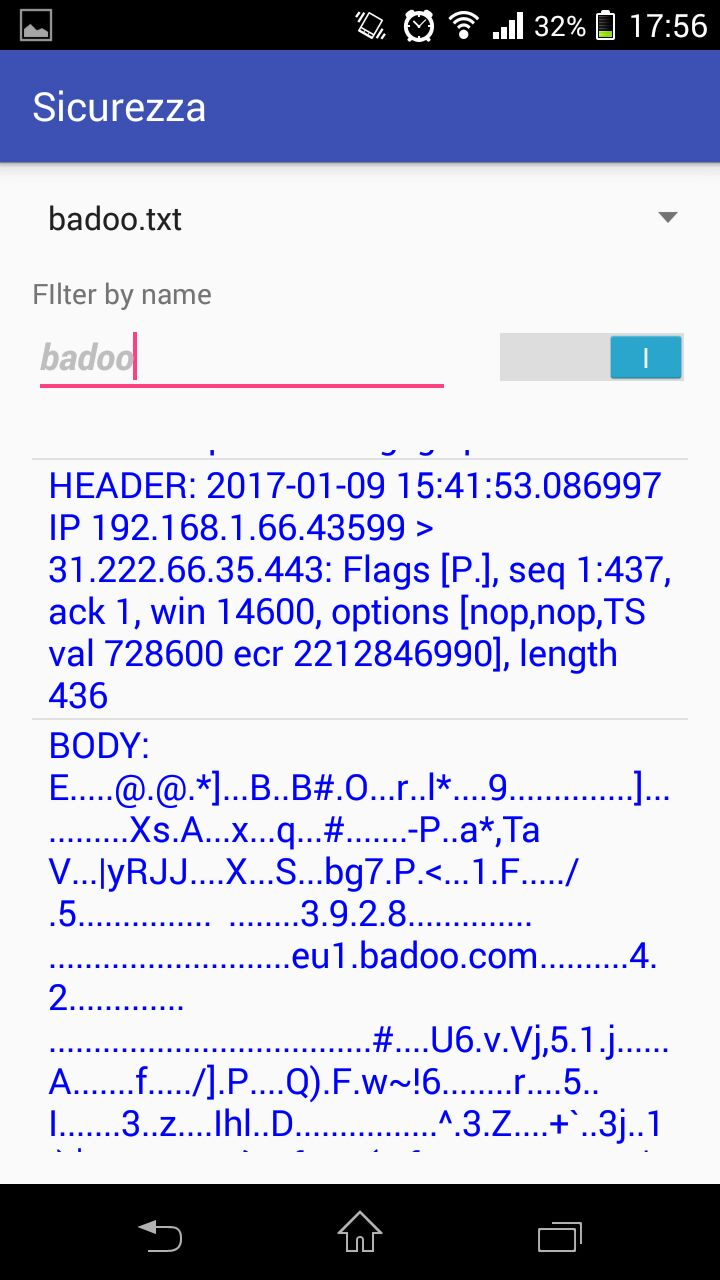
\includegraphics[scale=0.25]{./badoo.jpeg}}\qquad\qquad
\subfigure[Pacchetto Instagram\label{fig:instagram}]%
{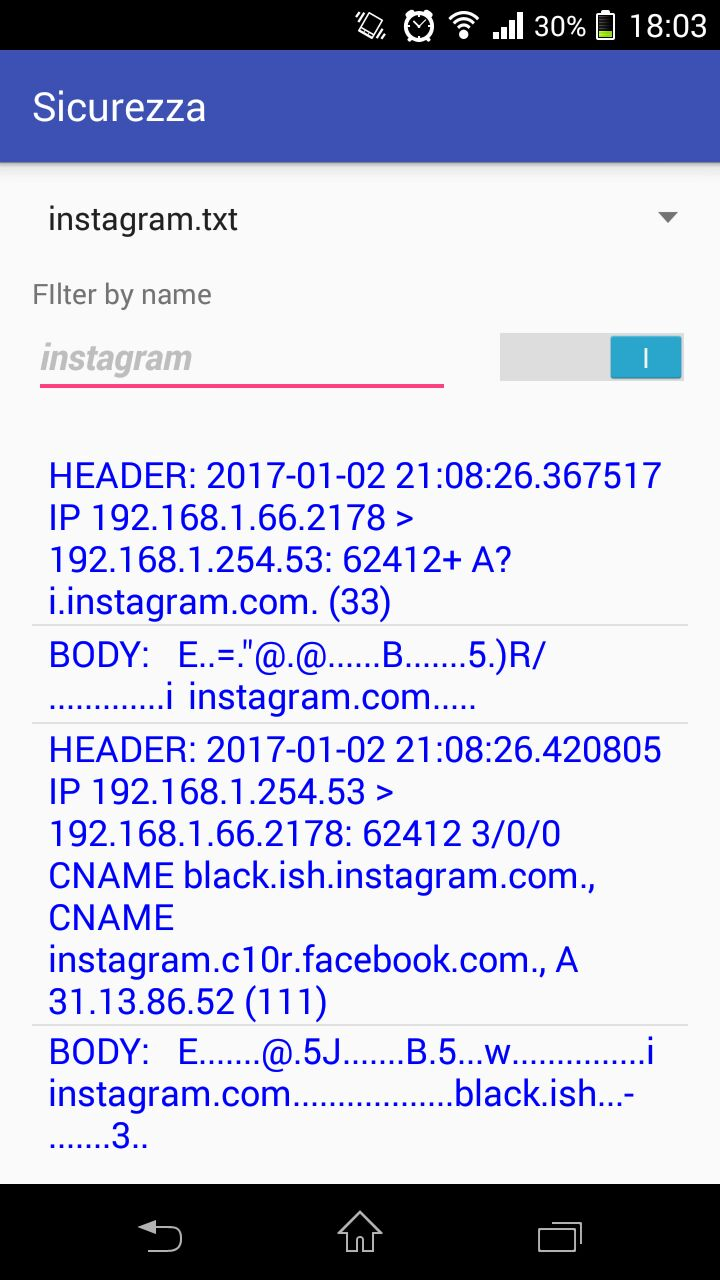
\includegraphics[scale=0.25]{./instagram.jpeg}}
\caption{Applicazioni Analizzate (1)\label{fig:app1}}
\end{figure} 

Inoltre nella tabella seguente vengono riassunti per ogni \textit{app} i \textit{security flaws} relativi all'\textit{header} ed al \textit{body} dei pacchetti (figure \ref{fig:table}).

\begin{figure}[htbp]
\centering%
\subfigure[Pacchetto Messenger\label{fig:messenger}]%
{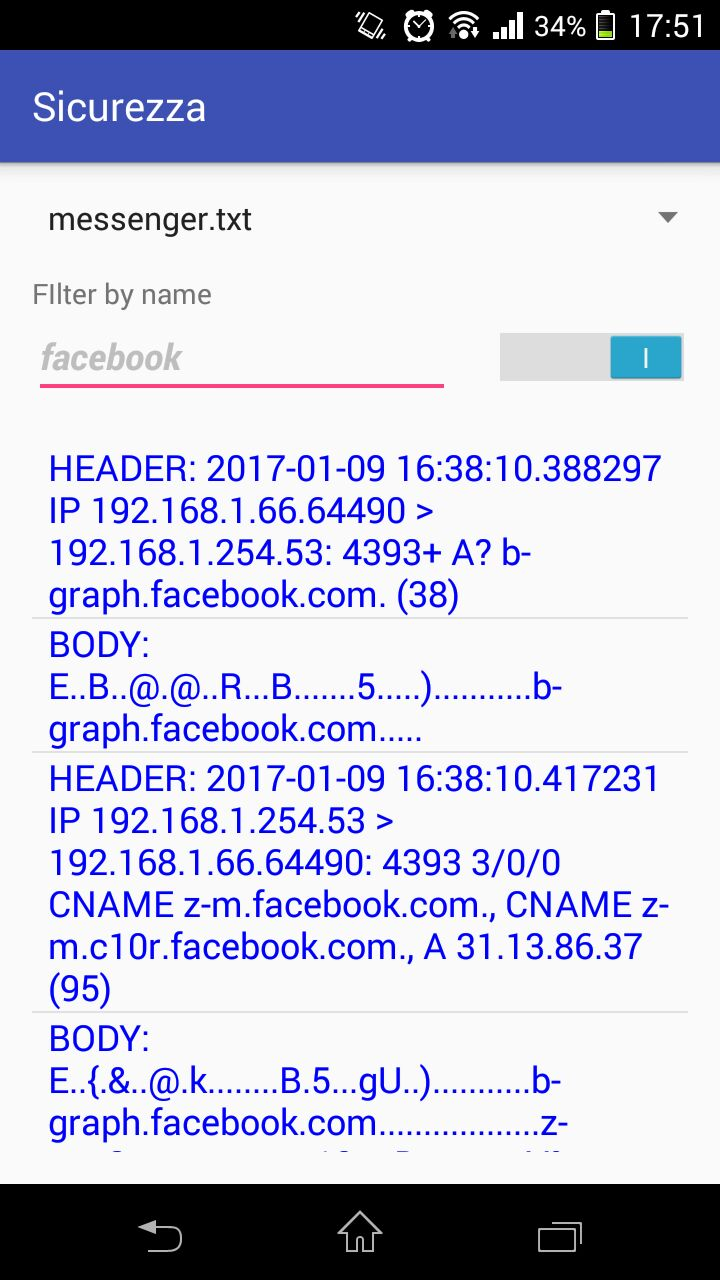
\includegraphics[scale=0.2]{./messenger.jpeg}}\qquad\qquad
\subfigure[Pacchetto Skype\label{fig:skype}]%
{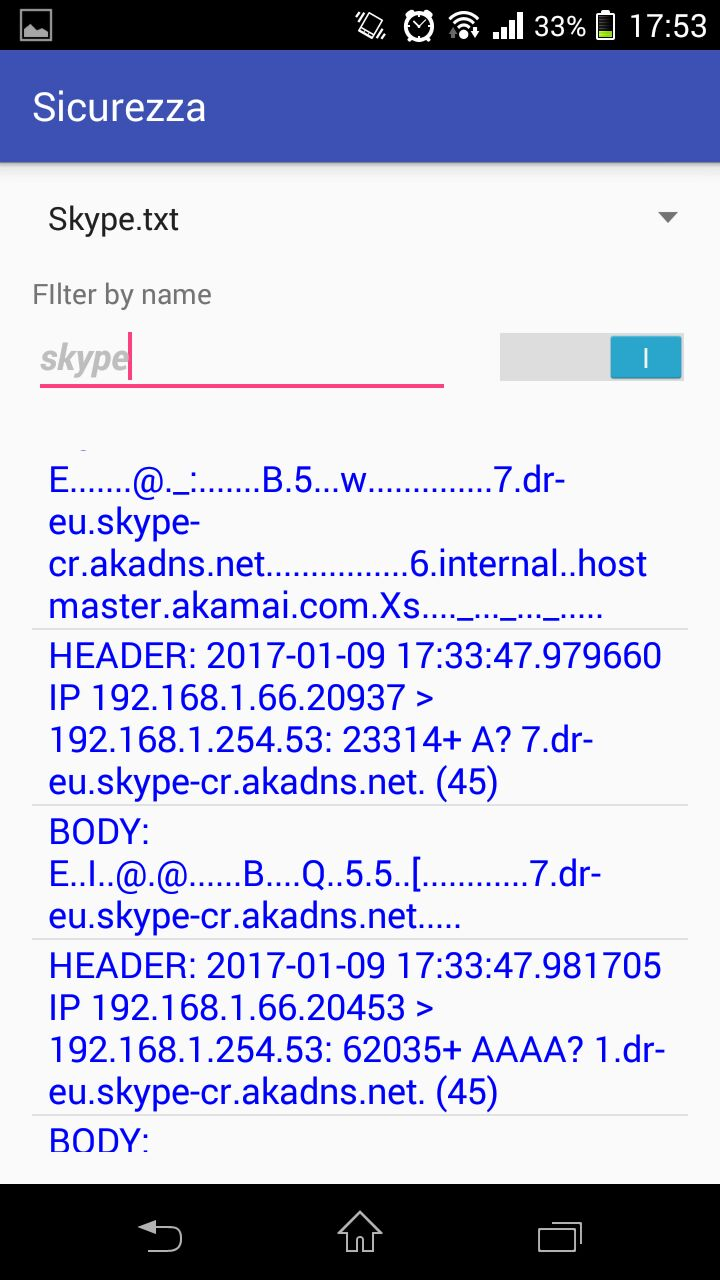
\includegraphics[scale=0.2]{./skype.jpeg}}
\\
\subfigure[Pacchetto Snapchat\label{fig:spapchat}]%
{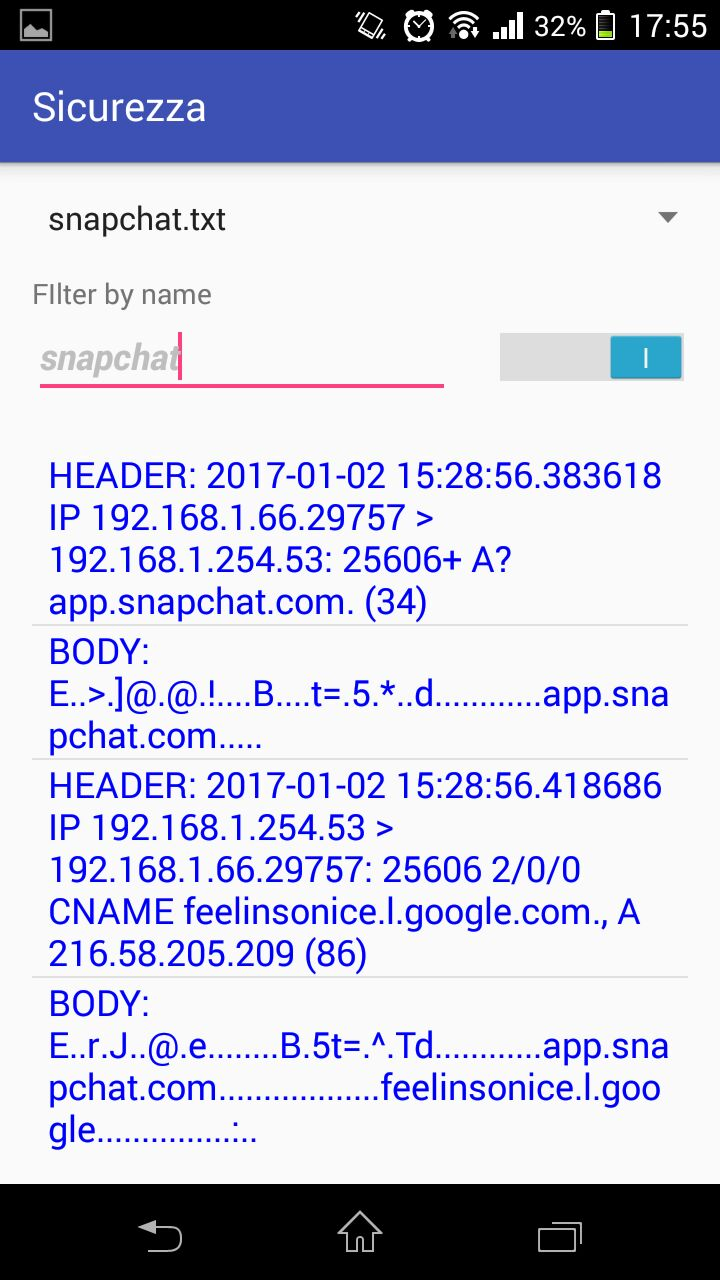
\includegraphics[scale=0.2]{./snap.jpeg}}
\caption{Applicazioni Analizzate (2)\label{fig:app2}}
\end{figure}

\begin{figure}
\centering
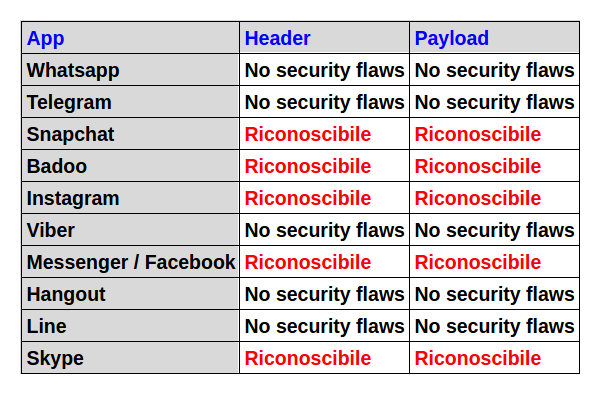
\includegraphics[scale=0.58]{./tabella.png}
\caption{Tabella delle applicazioni\label{fig:table}}
\end{figure}

\subsection{Test integrativi sulle modalit\'a di utilizzo della scheda di rete}
Per illustrare le differenze riguardanti la cattura dei pacchetti nell'utilizzo delle diverse modalit\'a di funzionamento della scheda di rete abbiamo effettuato test ulteriori su una piattaforma \textit{Linux} (\textit{Linux Mint 17.1 Cinnamon-64 bit}). Abbiamo condotto i test utilizzando la modalit\'a \textit{promiscua} e la modalit\'a \textit{monitor}. La modalit\'a promiscua \'e una modalit\'a di controllo in cui l'interfaccia di rete cablata o wireless filtra tutto il traffico di rete che l'unit\'a centrale (CPU) riesce ad analizzare; la sostanziale differenza \'e che la modalit\'a non promiscua analizza soltanto il frame che riceve o che destina. Adottando tale modalit\'a siamo stati in grado di catturare un sottoinsieme dei pacchetti \textit{multicast} identificati come appartenenti al protocollo \textit{IGMP}, destinati ad \textit{IP} della \textit{LAN} differenti dall'\textit{host tcpdump}. D'altro canto la modalit\'a \textit{monitor} permette la cattura di pacchetti della rete senza il bisogno di essere associati ad un \textit{access point} ma si applica esclusivamente a reti \textit{wireless}. Nel nostro test abbiamo notato una formattazione dei pacchetti totalmente differente da quella adottata dalla modalit\'a \textit{promiscua} che non ci ha permesso di isolare pacchetti appartenenti ad altri \textit{IP}. Un'altra motivazione che ci ha indotto a preferire la prima modalit\'a \'e legata al fatto che, nella modalit\'a \textit{monitor}, il \textit{wireless adapter} non controlla il \textit{CRC} dei pacchetti catturati e pertanto alcuni di questi pu\'o facilmente risultare corrotto, impedendo una corretta lettura.  
 
% Content

%----------------------------------------------------------------------------------------
%	CONCLUSION
%----------------------------------------------------------------------------------------

\section{Conclusioni e sviluppi futuri} % Major section
Sebbene la maggior parte delle applicazioni di messaggistica abbia fatto ricorso ad una forma di criptazione, alcune di esse presentano ancora alcune lacune in ambito di sicurezza. Infatti, come da noi dimostrato, \textit{app} come ad esempio \textit{Snapchat}, \textit{Badoo} e \textit{Instagram} espongono i propri pacchetti dati ad un elevato grado di riconoscibilit\'a. Un ipotetico attaccante, sebbene abbia un compito non banale quale la decriptazione di pacchetti, potrebbe pertanto distinguere da una grande mole di dati il suo target in maniera molto pi\'u immediata ed intuitiva. Tutto ci\'o dimostra che potrebbe essere necessario estendere la criptazione anche a porzioni del pacchetto che non rappresentano il \textit{payload}.\\
Per quanto riguarda lo \textit{sniffer}, un utilizzo pi\'u esteso delle opzioni della libreria \textit{tcpdump} potrebbe portare a delle migliorie in termini di personalizzazione della cattura. \textit{Tcpdump} infatti permette di combinare vari \textit{flag} in modo da ottenere una visualizzazione pacchetti il pi\'u vicina possibile al formato desiderato dall'utente. Invece dal punto di vista dell'applicazione \textit{Android} bisognerebbe apportare modifiche all'interfaccia grafica dell'\textit{Activity} di filtraggio ed aggiungervi opzioni utili ad evidenziare porzioni desiderate della lista dei pacchetti.



%----------------------------------------------------------------------------------------
%	BIBLIOGRAPHY
%----------------------------------------------------------------------------------------
\newpage

\begin{thebibliography}{99}
\bibitem{notes} \url{http://www.androidtcpdump.com}
\bibitem{notes} \url{http://www.tcpdump.org}
\bibitem{notes} \url{https://developer.android.com}
\bibitem{notes} \url{https://en.wikipedia.org}
\end{thebibliography}

\end{document}
